% Options for packages loaded elsewhere
\PassOptionsToPackage{unicode}{hyperref}
\PassOptionsToPackage{hyphens}{url}
\PassOptionsToPackage{dvipsnames,svgnames,x11names}{xcolor}
%

\documentclass{juliacon}

\usepackage{amsmath,amssymb}
\usepackage{setspace}
\usepackage{iftex}
\ifPDFTeX
  \usepackage[T1]{fontenc}
  \usepackage[utf8]{inputenc}
  \usepackage{textcomp} % provide euro and other symbols
\else % if luatex or xetex
  \usepackage{unicode-math}
  \defaultfontfeatures{Scale=MatchLowercase}
  \defaultfontfeatures[\rmfamily]{Ligatures=TeX,Scale=1}
\fi
\usepackage[]{tgtermes}
\ifPDFTeX\else  
    % xetex/luatex font selection
\fi
% Use upquote if available, for straight quotes in verbatim environments
\IfFileExists{upquote.sty}{\usepackage{upquote}}{}
\IfFileExists{microtype.sty}{% use microtype if available
  \usepackage[]{microtype}
  \UseMicrotypeSet[protrusion]{basicmath} % disable protrusion for tt fonts
}{}
\makeatletter
\@ifundefined{KOMAClassName}{% if non-KOMA class
  \IfFileExists{parskip.sty}{%
    \usepackage{parskip}
  }{% else
    \setlength{\parindent}{0pt}
    \setlength{\parskip}{6pt plus 2pt minus 1pt}}
}{% if KOMA class
  \KOMAoptions{parskip=half}}
\makeatother
\usepackage{xcolor}
\setlength{\emergencystretch}{3em} % prevent overfull lines
\setcounter{secnumdepth}{5}
% Make \paragraph and \subparagraph free-standing
\ifx\paragraph\undefined\else
  \let\oldparagraph\paragraph
  \renewcommand{\paragraph}[1]{\oldparagraph{#1}\mbox{}}
\fi
\ifx\subparagraph\undefined\else
  \let\oldsubparagraph\subparagraph
  \renewcommand{\subparagraph}[1]{\oldsubparagraph{#1}\mbox{}}
\fi


\providecommand{\tightlist}{%
  \setlength{\itemsep}{0pt}\setlength{\parskip}{0pt}}\usepackage{longtable,booktabs,array}
\usepackage{calc} % for calculating minipage widths
% Correct order of tables after \paragraph or \subparagraph
\usepackage{etoolbox}
\makeatletter
\patchcmd\longtable{\par}{\if@noskipsec\mbox{}\fi\par}{}{}
\makeatother
% Allow footnotes in longtable head/foot
\IfFileExists{footnotehyper.sty}{\usepackage{footnotehyper}}{\usepackage{footnote}}
\makesavenoteenv{longtable}
\usepackage{graphicx}
\makeatletter
\def\maxwidth{\ifdim\Gin@nat@width>\linewidth\linewidth\else\Gin@nat@width\fi}
\def\maxheight{\ifdim\Gin@nat@height>\textheight\textheight\else\Gin@nat@height\fi}
\makeatother
% Scale images if necessary, so that they will not overflow the page
% margins by default, and it is still possible to overwrite the defaults
% using explicit options in \includegraphics[width, height, ...]{}
\setkeys{Gin}{width=\maxwidth,height=\maxheight,keepaspectratio}
% Set default figure placement to htbp
\makeatletter
\def\fps@figure{htbp}
\makeatother
% definitions for citeproc citations
\NewDocumentCommand\citeproctext{}{}
\NewDocumentCommand\citeproc{mm}{%
  \begingroup\def\citeproctext{#2}\cite{#1}\endgroup}
\makeatletter
 % allow citations to break across lines
 \let\@cite@ofmt\@firstofone
 % avoid brackets around text for \cite:
 \def\@biblabel#1{}
 \def\@cite#1#2{{#1\if@tempswa , #2\fi}}
\makeatother
\newlength{\cslhangindent}
\setlength{\cslhangindent}{1.5em}
\newlength{\csllabelwidth}
\setlength{\csllabelwidth}{3em}
\newenvironment{CSLReferences}[2] % #1 hanging-indent, #2 entry-spacing
 {\begin{list}{}{%
  \setlength{\itemindent}{0pt}
  \setlength{\leftmargin}{0pt}
  \setlength{\parsep}{0pt}
  % turn on hanging indent if param 1 is 1
  \ifodd #1
   \setlength{\leftmargin}{\cslhangindent}
   \setlength{\itemindent}{-1\cslhangindent}
  \fi
  % set entry spacing
  \setlength{\itemsep}{#2\baselineskip}}}
 {\end{list}}
\usepackage{calc}
\newcommand{\CSLBlock}[1]{\hfill\break\parbox[t]{\linewidth}{\strut\ignorespaces#1\strut}}
\newcommand{\CSLLeftMargin}[1]{\parbox[t]{\csllabelwidth}{\strut#1\strut}}
\newcommand{\CSLRightInline}[1]{\parbox[t]{\linewidth - \csllabelwidth}{\strut#1\strut}}
\newcommand{\CSLIndent}[1]{\hspace{\cslhangindent}#1}

% Keywords command
\providecommand{\JCONkeywords}[1]
{
  \small	
  \section*{Keywords} #1
}

% Two-column table
% Lifted from https://github.com/quarto-journals/elsevier/blob/main/_extensions/elsevier/partials/_two-column-longtable.tex.
\usepackage{float}
\makeatletter
\let\oldlt\longtable
\let\endoldlt\endlongtable
\def\longtable{\@ifnextchar[\longtable@i \longtable@ii}
\def\longtable@i[#1]{\begin{figure}[H]
\onecolumn
\begin{minipage}{0.5\textwidth}
\oldlt[#1]
}
\def\longtable@ii{\begin{figure}[H]
\onecolumn
\begin{minipage}{0.5\textwidth}
\oldlt
}
\def\endlongtable{\endoldlt
\end{minipage}
\twocolumn
\end{figure}}
\makeatother

% Remove whitespace after paragraphs
\setlength{\parskip}{0pt}

% Bibliography stile
\bibliographystyle{juliacon}

\usepackage{orcidlink}
\definecolor{mypink}{RGB}{219, 48, 122}
\makeatletter
\@ifpackageloaded{caption}{}{\usepackage{caption}}
\AtBeginDocument{%
\ifdefined\contentsname
  \renewcommand*\contentsname{Table of contents}
\else
  \newcommand\contentsname{Table of contents}
\fi
\ifdefined\listfigurename
  \renewcommand*\listfigurename{List of Figures}
\else
  \newcommand\listfigurename{List of Figures}
\fi
\ifdefined\listtablename
  \renewcommand*\listtablename{List of Tables}
\else
  \newcommand\listtablename{List of Tables}
\fi
\ifdefined\figurename
  \renewcommand*\figurename{Figure}
\else
  \newcommand\figurename{Figure}
\fi
\ifdefined\tablename
  \renewcommand*\tablename{Table}
\else
  \newcommand\tablename{Table}
\fi
}
\@ifpackageloaded{float}{}{\usepackage{float}}
\floatstyle{ruled}
\@ifundefined{c@chapter}{\newfloat{codelisting}{h}{lop}}{\newfloat{codelisting}{h}{lop}[chapter]}
\floatname{codelisting}{Listing}
\newcommand*\listoflistings{\listof{codelisting}{List of Listings}}
\makeatother
\makeatletter
\makeatother
\makeatletter
\@ifpackageloaded{caption}{}{\usepackage{caption}}
\@ifpackageloaded{subcaption}{}{\usepackage{subcaption}}
\makeatother
\ifLuaTeX
  \usepackage{selnolig}  % disable illegal ligatures
\fi
\IfFileExists{bookmark.sty}{\usepackage{bookmark}}{\usepackage{hyperref}}
\IfFileExists{xurl.sty}{\usepackage{xurl}}{} % add URL line breaks if available
\urlstyle{same} % disable monospaced font for URLs
\hypersetup{
  pdftitle={Explaining Black-Box Models through Counterfactuals},
  pdfkeywords={Julia, Explainable Artificial
Intelligence, Counterfactual Explanations, Algorithmic Recourse},
  colorlinks=true,
  linkcolor={blue},
  filecolor={Maroon},
  citecolor={Blue},
  urlcolor={Blue},
  pdfcreator={LaTeX via pandoc}}


\title{Explaining Black-Box Models through Counterfactuals}

\author[1]{Patrick Altmeyer}
\author[1]{Arie van Deursen}
\author[1]{Cynthia C. S. Liem}
\affil[1]{Delft University of Technology}
\date{}
\begin{document}
\maketitle

% Abstract
\begin{abstract}

We present \texttt{CounterfactualExplanations.jl}: a package for
generating Counterfactual Explanations (CE) and Algorithmic Recourse
(AR) for black-box models in Julia. CE explain how inputs into a model
need to change to yield specific model predictions. Explanations that
involve realistic and actionable changes can be used to provide AR: a
set of proposed actions for individuals to change an undesirable outcome
for the better. In this article, we discuss the usefulness of CE for
Explainable Artificial Intelligence and demonstrate the functionality of
our package. The package is straightforward to use and designed with a
focus on customization and extensibility. We envision it to one day be
the go-to place for explaining arbitrary predictive models in Julia
through a diverse suite of counterfactual generators.
\end{abstract}

% Keywords
\JCONkeywords{Julia, Explainable Artificial Intelligence, Counterfactual
Explanations, Algorithmic Recourse}

% Hypersetup
\hypersetup{
    pdftitle = {Explaining Black-Box Models through Counterfactuals},
    pdfsubject = {JuliaCon \@year Proceedings},
    pdfauthor = {},
    pdfkeywords = {Julia, Explainable Artificial
Intelligence, Counterfactual Explanations, Algorithmic Recourse},
}

\setcounter{page}{1}

\setstretch{1}
\section{Introduction}\label{sec-intro}

Machine Learning models like Deep Neural Networks have become so complex
and opaque over recent years that they are generally considered
black-box systems. This lack of transparency exacerbates several other
problems typically associated with these models: they tend to be
unstable (\citeproc{ref-goodfellow2014explaining}{Goodfellow, Shlens,
and Szegedy 2014}), encode existing biases
(\citeproc{ref-buolamwini2018gender}{Buolamwini and Gebru 2018}) and
learn representations that are surprising or even counter-intuitive from
a human perspective (\citeproc{ref-buolamwini2018gender}{Buolamwini and
Gebru 2018}). Nonetheless, they often form the basis for data-driven
decision-making systems in real-world applications.

As others have pointed out, this scenario gives rise to an undesirable
principal-agent problem involving a group of principals---i.e.~human
stakeholders---that fail to understand the behaviour of their
agent---i.e.~the black-box system (\citeproc{ref-borch2022machine}{Borch
2022}). The group of principals may include programmers, product
managers and other decision-makers who develop and operate the system as
well as those individuals ultimately subject to the decisions made by
the system. In practice, decisions made by black-box systems are
typically left unchallenged since the group of principals cannot
scrutinize them:

\begin{quote}
``You cannot appeal to (algorithms). They do not listen. Nor do they
bend.'' (\citeproc{ref-oneil2016weapons}{O'Neil 2016})
\end{quote}

In light of all this, a quickly growing body of literature on
Explainable Artificial Intelligence (XAI) has emerged. Counterfactual
Explanations fall into this broad category. They can help human
stakeholders make sense of the systems they develop, use or endure: they
explain how inputs into a system need to change for it to produce
different decisions. Explainability benefits internal as well as
external quality assurance. Explanations that involve plausible and
actionable changes can be used for Algorithmic Recourse (AR): they offer
the group of principals a way to not only understand their agent's
behaviour but also adjust or react to it.

The availability of open-source software to explain black-box models
through counterfactuals is still limited. Through the work presented
here, we aim to close that gap and thereby contribute to broader
community efforts towards XAI. We envision this package to one day be
the go-to place for Counterfactual Explanations in Julia. Thanks to
Julia's unique support for interoperability with foreign programming
languages we believe that this library may also benefit the broader
machine learning and data science community.

Our package provides a simple and intuitive interface to generate CE for
many standard classification models trained in Julia, as well as in
Python and R. It comes with detailed documentation involving various
illustrative example datasets, models and counterfactual generators for
binary and multi-class prediction tasks. A carefully designed package
architecture allows for a seamless extension of the package
functionality through custom generators and models.

The remainder of this article is structured as follows:
Section~\ref{sec-related} presents related work on XAI as well as a
brief overview of the methodological framework underlying CE.
Section~\ref{sec-arch} introduces the Julia package and its high-level
architecture. Section~\ref{sec-use} presents several basic and advanced
usage examples. In Section~\ref{sec-custom} we demonstrate how the
package functionality can be customized and extended. To illustrate its
practical usability, we explore examples involving real-world data in
Section~\ref{sec-emp}. Finally, we also discuss the current limitations
of our package, as well as its future outlook in
Section~\ref{sec-outlook}. Section~\ref{sec-conclude} concludes.

\section{Background and related work}\label{sec-related}

In this section, we first briefly introduce the broad field of
Explainable AI, before narrowing it down to Counterfactual Explanations.
We introduce the methodological framework and finally point to existing
open-source software.

\subsection{Literature on Explainable
AI}\label{literature-on-explainable-ai}

The field of XAI is still relatively young and made up of a variety of
subdomains, definitions, concepts and taxonomies. Covering all of these
is beyond the scope of this article, so we will focus only on high-level
concepts. The following literature surveys provide more detail: Arrieta
et al.~(2020) provide a broad overview of XAI
(\citeproc{ref-arrieta2020explainable}{Arrieta et al. 2020}); Fan et
al.~(2020) focus on explainability in the context of deep learning
(\citeproc{ref-fan2020interpretability}{Fan, Xiong, and Wang 2020}); and
finally, Karimi et al.~(2020) (\citeproc{ref-karimi2020survey}{Karimi,
Barthe, et al. 2020}) and Verma et al.~(2020) Verma, Dickerson, and
Hines (\citeproc{ref-verma2020counterfactual}{2020}) offer detailed
reviews of the literature on Counterfactual Explanations and Algorithmic
Recourse (see also Molnar (\citeproc{ref-molnar2020interpretable}{2020})
and Varshney (\citeproc{ref-varshney2022trustworthy}{2022})). Miller
(2019) explicitly discusses the concept of explainability from the
perspective of a social scientist
(\citeproc{ref-miller2019explanation}{Miller 2019}).

The first broad distinction we want to make here is between
\textbf{Interpretable} and \textbf{Explainable} AI. These terms are
often used interchangeably, but this can lead to confusion. We find the
distinction made in Rudin (\citeproc{ref-rudin2019stop}{2019}) useful:
Interpretable AI involves models that are inherently interpretable and
transparent such as general additive models (GAM), decision trees and
rule-based models; Explainable AI involves models that are not
inherently interpretable but require additional tools to be explainable
to humans. Examples of the latter include Ensembles, Support Vector
Machines and Deep Neural Networks. Some would argue that we best avoid
the second category of models altogether and instead focus solely on
interpretable AI Rudin (\citeproc{ref-rudin2019stop}{2019}). While we
agree that initial efforts should always be geared towards interpretable
models, avoiding black boxes altogether would entail missed
opportunities and anyway is probably not very realistic at this point.
For that reason, we expect the need for XAI to persist in the medium
term. Explainable AI can further be broadly divided into \textbf{global}
and \textbf{local} explainability: the former is concerned with
explaining the average behaviour of a model, while the latter involves
explanations for individual predictions
(\citeproc{ref-molnar2020interpretable}{Molnar 2020}). Tools for global
explainability include partial dependence plots (PDP), which involve the
computation of marginal effects through Monte Carlo, and global
surrogates. A surrogate model is an interpretable model that is trained
to explain the predictions of a black-box model.

Counterfactual Explanations fall into the category of local methods:
they explain how individual predictions change in response to individual
feature perturbations. Among the most popular alternatives to
Counterfactual Explanations are local surrogate explainers including
Local Interpretable Model-agnostic Explanations (LIME) and Shapley
additive explanations (SHAP). Since explanations produced by LIME and
SHAP typically involve simple feature importance plots, they arguably
rely on reasonably interpretable features at the very least. Contrary to
Counterfactual Explanations, for example, it is not obvious how to apply
LIME and SHAP to high-dimensional image data. Nonetheless, local
surrogate explainers are among the most widely used XAI tools today,
potentially because they are easy to interpret and implemented in
popular programming languages. Proponents of surrogate explainers also
commonly mention that there is a straightforward way to assess their
reliability: a surrogate model that generates predictions in line with
those produced by the black-box model is said to have high
\textbf{fidelity} and therefore considered reliable. As intuitive as
this notion may be, it also points to an obvious shortfall of surrogate
explainers: even a high-fidelity surrogate model that produces the same
predictions as the black-box model 99 per cent of the time is useless
and potentially misleading for every 1 out of 100 individual
predictions.

A recent study has shown that even experienced data scientists tend to
put too much trust in explanations produced by LIME and SHAP
(\citeproc{ref-kaur2020interpreting}{Kaur et al. 2020}). Another recent
work has shown that both methods can be easily fooled: they depend on
random input perturbations, a property that can be abused by adverse
agents to essentially whitewash strongly biased black-box models
(\citeproc{ref-slack2020fooling}{Slack et al. 2020}). In related work,
the same authors find that while gradient-based Counterfactual
Explanations can also be manipulated, there is a straightforward way to
protect against this in practice
(\citeproc{ref-slack2021counterfactual}{Slack et al. 2021}). In the
context of quality assessment, it is also worth noting that---contrary
to surrogate explainers---CE always achieve full fidelity by
construction: counterfactuals are searched with respect to the black-box
classifier, not some proxy for it. That being said, CE should also be
used with care and research around them is still in its early stages.

\subsection{A framework for Counterfactual
Explanations}\label{sec-method}

Counterfactual search involves feature perturbations: we are interested
in understanding how we need to change individual attributes in order to
change the model output to a desired value or label
(\citeproc{ref-molnar2020interpretable}{Molnar 2020}). Typically the
underlying methodology is presented in the context of binary
classification: \(M: \mathcal{X} \mapsto \mathcal{Y}\) where
\(\mathcal{X}\subset\mathbb{R}^D\) and \(\mathcal{Y}=\{0,1\}\). Further,
let \(t=1\) be the target class and let \(x\) denote the factual feature
vector of some individual sample outside of the target class, so
\(y=M(x)=0\). We follow this convention here, though it should be noted
that the ideas presented here also carry over to multi-class problems
and regression (\citeproc{ref-molnar2020interpretable}{Molnar 2020}).

The counterfactual search objective originally proposed by Wachter,
Mittelstadt, and Russell
(\citeproc{ref-wachter2017counterfactual}{2017}) is as follows

\begin{equation}\phantomsection\label{eq-obj}{
\min_{x^\prime \in \mathcal{X}} h(x^\prime) \ \ \ \mbox{s. t.} \ \ \ M(x^\prime) = t
}\end{equation}

where \(h(\cdot)\) quantifies how complex or costly it is to go from the
factual \(x\) to the counterfactual \(x^\prime\). To simplify things we
can restate this constrained objective as the following unconstrained
and differentiable problem:

\begin{equation}\phantomsection\label{eq-solution}{
x^\prime = \arg \min_{x^\prime}  \ell(M(x^\prime),t) + \lambda h(x^\prime)
}\end{equation}

Here \(\ell\) denotes some loss function targeting the deviation between
the target label and the predicted label and \(\lambda\) governs the
strength of the complexity penalty. Provided we have gradient access for
the black-box model \(M\) the solution to this problem can be found
through gradient descent. This generic framework lays the foundation for
most state-of-the-art approaches to counterfactual search and is also
used as the baseline approach in our package. The hyperparameter
\(\lambda\) is typically tuned through grid search or in some sense
pre-determined by the nature of the problem. Conventional choices for
\(\ell\) include margin-based losses like cross-entropy loss and hinge
loss. It is worth pointing out that the loss function is typically
computed with respect to logits rather than predicted probabilities, a
convention that we have chosen to follow.\footnote{Implementations of
  loss functions with respect to logits are often numerically more
  stable. For example, the \texttt{logitbinarycrossentropy(ŷ,\ y)}
  implementation in \texttt{Flux.Losses} (used here) is more stable than
  the mathematically equivalent \texttt{binarycrossentropy(ŷ,\ y)}.}

Numerous extensions to this simple approach have been developed since CE
were first proposed in 2017 (see Verma, Dickerson, and Hines
(\citeproc{ref-verma2020counterfactual}{2020}) and
(\citeproc{ref-karimi2020survey}{Karimi, Barthe, et al. 2020}) for
surveys). The various approaches largely differ in that they use
different flavours of search objective defined in
Equation~\ref{eq-solution}. Different penalties are often used to
address many of the desirable properties of effective CE that have been
set out. These desiderata include: \textbf{proximity} --- the distance
between factual and counterfactual features should be small
(\citeproc{ref-wachter2017counterfactual}{Wachter, Mittelstadt, and
Russell 2017}); \textbf{actionability} --- the proposed recourse should
be actionable Poyiadzi et al. (\citeproc{ref-poyiadzi2020face}{2020});
\textbf{plausibility} --- the counterfactual explanation should be
plausible to a human Schut et al.
(\citeproc{ref-schut2021generating}{2021}); \textbf{sparsity} --- the
counterfactual explanation should involve as few individual feature
changes as possible (\citeproc{ref-schut2021generating}{Schut et al.
2021}); \textbf{robustness} --- the counterfactual explanation should be
robust to domain and model shifts
(\citeproc{ref-upadhyay2021robust}{Upadhyay, Joshi, and Lakkaraju
2021}); \textbf{diversity} --- ideally multiple diverse counterfactuals
should be provided (\citeproc{ref-mothilal2020explaining}{Mothilal,
Sharma, and Tan 2020}); and \textbf{causality} --- counterfactuals
should respect the structural causal model underlying the data
generating process Karimi, Schölkopf, and Valera
(\citeproc{ref-karimi2021algorithmic}{2021}).

Beyond gradient-based counterfactual search, which has been the main
focus in our development so far, various methodologies have been
proposed that can handle non-differentiable models like decision trees.
We have implemented some of these approaches and will discuss them
further in Section~\ref{sec-gen}.

\subsection{Existing software}\label{existing-software}

To the best of our knowledge, the package introduced here provides the
first implementation of Counterfactual Explanations in Julia and
therefore represents a novel contribution to the community. As for other
programming languages, we are only aware of one other unifying
framework: the Python library
\href{https://carla-counterfactual-and-recourse-library.readthedocs.io/en/latest/?badge=latest}{CARLA}
(\citeproc{ref-pawelczyk2021carla}{Pawelczyk et al. 2021}).\footnote{While
  we were writing this paper, the \texttt{R} package
  \texttt{counterfactuals} was released
  (\citeproc{ref-dandl2023counterfactuals}{Dandl et al. 2023}). The
  developers seem to also envision a unifying framework, but the project
  appears to still be in its early stages.} In addition to that, there
exists open-source code for some specific approaches to CE that have
been proposed in recent years. The approach-specific implementations
that we have been able to find are generally well-documented, but
exclusively in Python. For example, a PyTorch implementation of a greedy
generator for Bayesian models proposed in Schut et al.
(\citeproc{ref-schut2021generating}{2021}) has been released. As another
example, the popular \href{https://github.com/interpretml}{InterpretML}
library includes an implementation of a diverse counterfactual generator
(\citeproc{ref-mothilal2020explaining}{Mothilal, Sharma, and Tan 2020}).

Generally speaking, software development in the space of XAI has largely
focused on various global methods and surrogate explainers:
implementations of PDP, LIME and SHAP are available for both Python
(e.g.~\href{https://github.com/marcotcr/lime}{\texttt{lime}},
\href{https://github.com/slundberg/shap}{\texttt{shap}}) and R
(e.g.~\href{https://cran.r-project.org/web/packages/lime/index.html}{\texttt{lime}},
\href{https://cran.r-project.org/web/packages/lime/index.html}{\texttt{iml}},
\href{https://modeloriented.github.io/shapper/}{\texttt{shapper}},
\href{https://github.com/bgreenwell/fastshap}{\texttt{fastshap}}). In
the Julia space, there exist two packages related to XAI: firstly,
\href{https://github.com/nredell/ShapML.jl}{\texttt{ShapML.jl}}, which
provides a fast implementation of SHAP; and, secondly,
\href{https://github.com/adrhill/ExplainableAI.jl}{\texttt{ExplainableAI.jl}},
which enables users to easily visualise gradients and activation maps
for \texttt{Flux.jl} models. We also should not fail to mention the
comprehensive
\href{https://docs.interpretable.ai/stable/IAIBase/data/}{Interpretable
AI} infrastructure, which focuses exclusively on interpretable models.

Arguably the current availability of tools for explaining black-box
models in Julia is limited, but it appears that the community is
invested in changing that. The team behind \texttt{MLJ.jl}, for example,
recruited contributors for a project about both Interpretable and
Explainable AI in 2022.\footnote{For details, see the Google Summer of
  Code 2022 project proposal:
  \url{https://julialang.org/jsoc/gsoc/MLJ/\#interpretable_machine_learning_in_julia}.}
With our work on Counterfactual Explanations we hope to contribute to
these efforts. We think that because of its unique transparency the
Julia language naturally lends itself towards building Trustworthy AI
systems.

\section{\texorpdfstring{Introducing:
\texttt{CounterfactualExplanations.jl}}{Introducing: CounterfactualExplanations.jl}}\label{sec-arch}

Figure~\ref{fig-arch} provides an overview of the package architecture.
It is built around two core modules that are designed to be as
extensible as possible through dispatch: 1) \texttt{Models} is concerned
with making any arbitrary model compatible with the package; 2)
\texttt{Generators} is used to implement counterfactual search
algorithms. The core function of the
package---\texttt{generate\_counterfactual}---uses an instance of type
\texttt{\textless{}:AbstractFittedModel} produced by the \texttt{Models}
module and an instance of type \texttt{\textless{}:AbstractGenerator}
produced by the \texttt{Generators} module. Relating this to the
methodology outlined in Section~\ref{sec-method}, the former instance
corresponds to the model \(M\), while the latter defines the rules for
the counterfactual search (Equation~\ref{eq-solution}).

\begin{figure}

\centering{

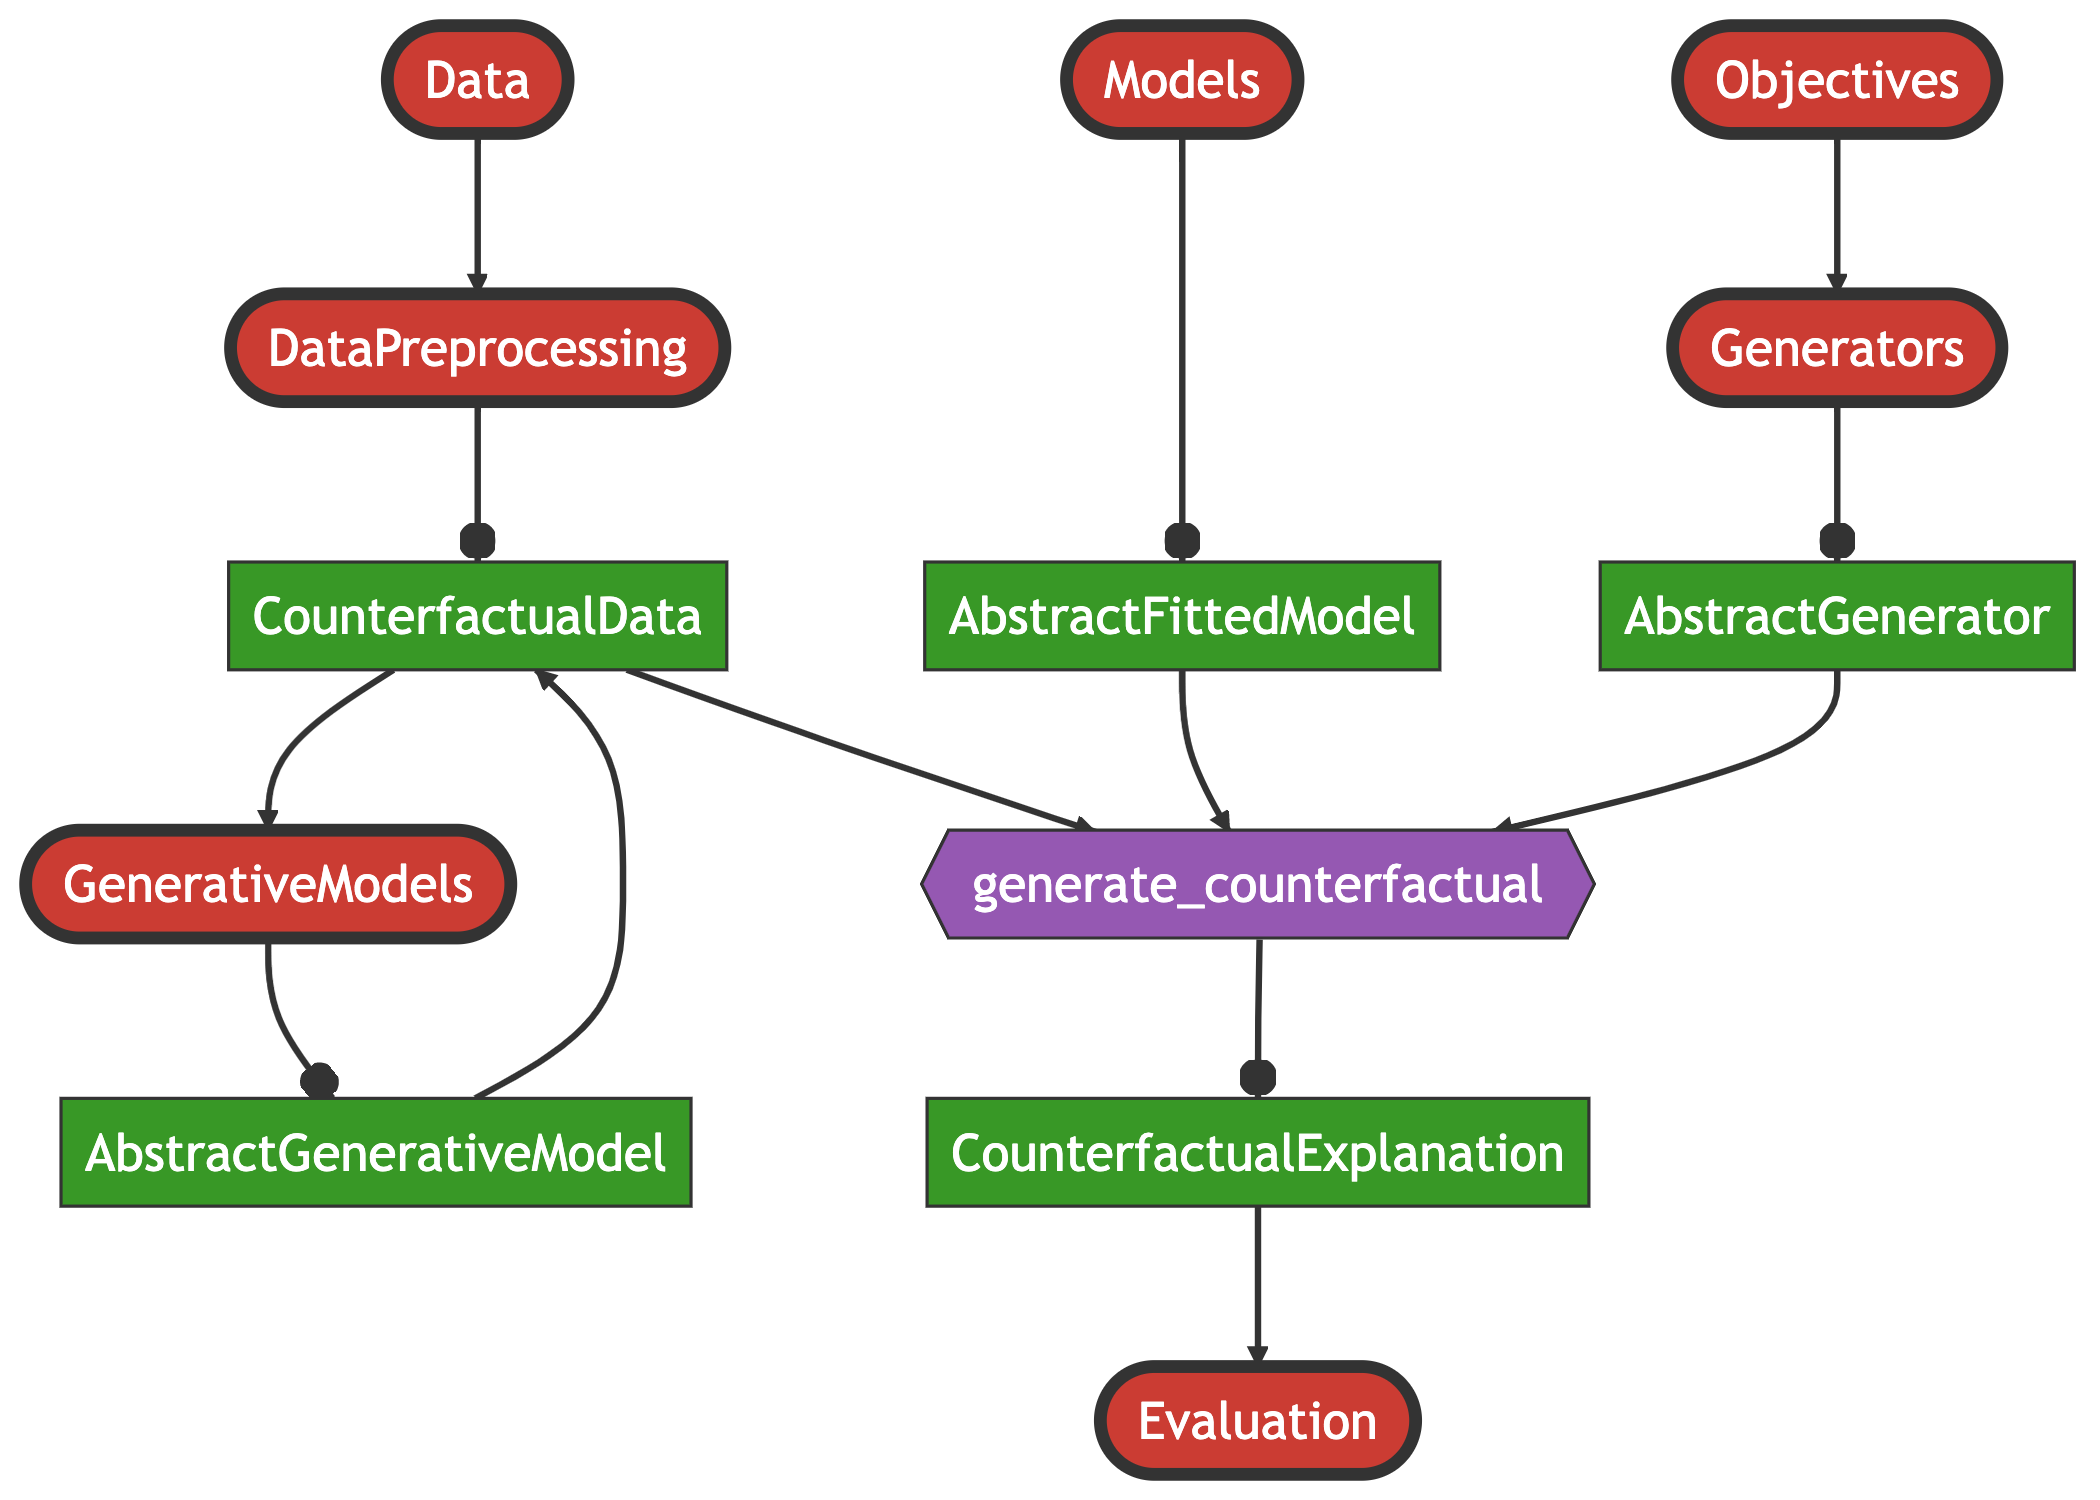
\includegraphics[width=3.33333in,height=2.38095in]{www/pkg_architecture.png}

}

\caption{\label{fig-arch}High-level schematic overview of package
architecture. Modules are shown in red, structs in green and functions
in purple.}

\end{figure}%

\subsection{Models}\label{models}

The package currently offers native support for models built and trained
in \href{https://fluxml.ai/}{Flux} (\citeproc{ref-innes2018flux}{Innes
2018}) as well as a small subset of models made available through
\href{https://alan-turing-institute.github.io/MLJ.jl/dev/}{MLJ}
(\citeproc{ref-blaom2020mlj}{Blaom et al. 2020}). While in general it is
assumed that users resort to this package to explain their pre-trained
models, we provide a simple API call to train the following
\href{https://juliatrustworthyai.github.io/CounterfactualExplanations.jl/v0.1/tutorials/model_catalogue/}{models}:

\begin{itemize}
\tightlist
\item
  Linear Classifier (Logistic Regression and Multinomial Logit)
\item
  Multi-Layer Perceptron (Deep Neural Network)
\item
  Deep Ensemble Lakshminarayanan, Pritzel, and Blundell
  (\citeproc{ref-lakshminarayanan2016simple}{2016})
\item
  Decision Tree, Random Forest, Gradient Boosted Trees
\end{itemize}

As we demonstrate below, it is straightforward to extend the package
through custom models. Support for \texttt{torch} models trained in
Python or R is also available.\footnote{We are currently relying on
  \texttt{PythonCall.jl} and \texttt{RCall.jl} and this functionality is
  still somewhat brittle. Since this is more of an edge case, we may
  move this feature into its own package in the future.}

\subsection{Generators}\label{sec-gen}

A large and growing number of counterfactual
\href{https://juliatrustworthyai.github.io/CounterfactualExplanations.jl/v0.1/explanation/generators/overview/}{generators}
have already been implemented in our package (Table~\ref{tbl-gen}). At a
high level, we distinguish generators in terms of their compatible model
types, their default search space, and their composability. All
``gradient-based'' generators are compatible with differentiable models,
e.g.~\texttt{Flux} and \texttt{torch}, while ``tree-based'' generators
are only applicable to models that involve decision trees. Concerning
the search space, it is possible to search counterfactuals in a
lower-dimensional latent embedding of the feature space that implicitly
encodes the data-generating process (DGP). To learn the latent
embedding, existing work has typically relied on generative models or
existing causal knowledge Karimi, Schölkopf, and Valera
(\citeproc{ref-karimi2021algorithmic}{2021}). While this notion is
compatible with all of our gradient-based generators, only some
generators search a latent space by default. Finally, composability
implies that the given generator can be blended with any other
composable generator, which we discuss in Section~\ref{sec-gen-comp}.

Beyond these broad technical distinctions, generators largely differ in
terms of how they address the various desiderata mentioned above:
\emph{ClapROAR} aims to preserve the classifier, i.e.~to generate
counterfactuals that are robust to endogenous model shifts
(\citeproc{ref-altmeyer2023endogenous}{Altmeyer et al. 2023});
\emph{CLUE} searches plausible counterfactuals in the latent embedding
of a generative model by explicitly minimising predictive entropy
(\citeproc{ref-antoran2020getting}{Antorán et al. 2020}); \emph{DiCE} is
designed to generate multiple, maximally diverse counterfactuals
(\citeproc{ref-mothilal2020explaining}{Mothilal, Sharma, and Tan 2020});
\emph{FeatureTweak} leverages the internals of decision trees to search
counterfactuals on a feature-by-feature basis, finding the
counterfactual that tweaks the features in the least costly way
(\citeproc{ref-tolomei2017interpretable}{Tolomei et al. 2017});
\emph{Gravitational} aims to generate plausible and robust
counterfactuals by minimising the distance to observed samples in the
target class (\citeproc{ref-altmeyer2023endogenous}{Altmeyer et al.
2023}); \emph{Greedy} aims to generate plausible counterfactuals by
implicitly minimising predictive uncertainty of Bayesian classifiers
(\citeproc{ref-schut2021generating}{Schut et al. 2021});
\emph{GrowingSpheres} is model-agnostic, relying solely on identifying
nearest neighbours of counterfactuals in the target class by gradually
increasing the search radius and then moving counterfactuals in that
direction(\citeproc{ref-laugel2017inversea}{Laugel et al. 2017});
\emph{PROBE} generates probabilistically robust counterfactuals
(\citeproc{ref-pawelczyk2022probabilistically}{Pawelczyk et al. 2022});
\emph{REVISE} addresses the need for plausibility by searching
counterfactuals in the latent embedding of a Variational Autoencoder
(VAE) (\citeproc{ref-joshi2019realistic}{Joshi et al. 2019});
\emph{Wachter} is the baseline approach that only penalises the distance
to the original sample
(\citeproc{ref-wachter2017counterfactual}{Wachter, Mittelstadt, and
Russell 2017}).

\begin{longtable}[]{@{}
  >{\raggedright\arraybackslash}p{(\columnwidth - 6\tabcolsep) * \real{0.2500}}
  >{\raggedright\arraybackslash}p{(\columnwidth - 6\tabcolsep) * \real{0.2500}}
  >{\raggedright\arraybackslash}p{(\columnwidth - 6\tabcolsep) * \real{0.2500}}
  >{\raggedright\arraybackslash}p{(\columnwidth - 6\tabcolsep) * \real{0.2500}}@{}}
\caption{Overview of implemented counterfactual
generators.}\label{tbl-gen}\tabularnewline
\toprule\noalign{}
\begin{minipage}[b]{\linewidth}\raggedright
Generator
\end{minipage} & \begin{minipage}[b]{\linewidth}\raggedright
Model Type
\end{minipage} & \begin{minipage}[b]{\linewidth}\raggedright
Search Space
\end{minipage} & \begin{minipage}[b]{\linewidth}\raggedright
Composable
\end{minipage} \\
\midrule\noalign{}
\endfirsthead
\toprule\noalign{}
\begin{minipage}[b]{\linewidth}\raggedright
Generator
\end{minipage} & \begin{minipage}[b]{\linewidth}\raggedright
Model Type
\end{minipage} & \begin{minipage}[b]{\linewidth}\raggedright
Search Space
\end{minipage} & \begin{minipage}[b]{\linewidth}\raggedright
Composable
\end{minipage} \\
\midrule\noalign{}
\endhead
\bottomrule\noalign{}
\endlastfoot
ClaPROAR (\citeproc{ref-altmeyer2023endogenous}{Altmeyer et al. 2023}) &
gradient based & feature & yes \\
CLUE (\citeproc{ref-antoran2020getting}{Antorán et al. 2020}) & gradient
based & latent & yes \\
DiCE (\citeproc{ref-mothilal2020explaining}{Mothilal, Sharma, and Tan
2020}) & gradient based & feature & yes \\
FeatureTweak (\citeproc{ref-tolomei2017interpretable}{Tolomei et al.
2017}) & tree based & feature & no \\
Gravitational (\citeproc{ref-altmeyer2023endogenous}{Altmeyer et al.
2023}) & gradient based & feature & yes \\
Greedy (\citeproc{ref-schut2021generating}{Schut et al. 2021}) &
gradient based & feature & yes \\
GrowingSpheres (\citeproc{ref-laugel2017inversea}{Laugel et al. 2017}) &
agnostic & feature & no \\
PROBE (\citeproc{ref-pawelczyk2022probabilistically}{Pawelczyk et al.
2022}) & gradient based & feature & no \\
REVISE (\citeproc{ref-joshi2019realistic}{Joshi et al. 2019}) & gradient
based & latent & yes \\
Wachter (\citeproc{ref-wachter2017counterfactual}{Wachter, Mittelstadt,
and Russell 2017}) & gradient based & feature & yes \\
\end{longtable}

\subsection{Data Catalogue}\label{data-catalogue}

To allow researchers and practitioners to test and compare
counterfactual generators, the package ships with
\href{https://juliatrustworthyai.github.io/CounterfactualExplanations.jl/v0.1/tutorials/data_catalogue/}{catalogues}
of pre-processed synthetic and real-world benchmark datasets from
different domains. Real-world datasets include:

\begin{itemize}
\tightlist
\item
  Adult Census (\citeproc{ref-becker1996adult}{Barry Becker 1996})
\item
  California Housing (\citeproc{ref-pace1997sparse}{Pace and Barry
  1997})
\item
  CIFAR10 (\citeproc{ref-krizhevsky2009learning}{Krizhevsky 2009})
\item
  German Credit (\citeproc{ref-hoffman1994german}{Hoffman 1994})
\item
  Give Me Some Credit (\citeproc{ref-kaggle2011give}{Kaggle 2011})
\item
  MNIST (\citeproc{ref-lecun1998mnist}{LeCun 1998}) and Fashion MNIST
  (\citeproc{ref-xiao2017fashion}{Xiao, Rasul, and Vollgraf 2017})
\item
  UCI defaultCredit (\citeproc{ref-yeh2009comparisons}{Yeh and Lien
  2009})
\end{itemize}

Custom datasets can also be easily preprocessed as explained in the
\href{https://juliatrustworthyai.github.io/CounterfactualExplanations.jl/v0.1/tutorials/data_preprocessing/}{documentation}.

\subsection{Plotting}\label{plotting}

The package also extends common \texttt{Plots.jl} methods to facilitate
the visualization of results. Calling the generic \texttt{plot()} method
on an instance of type \texttt{\textless{}:CounterfactualExplanation},
for example, generates a plot visualizing the entire counterfactual path
in the feature space\footnote{For multi-dimensional input data, standard
  dimensionality reduction techniques are used to compress the data. In
  this case, the classifier's decision boundary is approximated through
  a Nearest Neighbour model. This is still somewhat experimental and
  will be improved in the future.}. We will see several examples of this
below.

\section{Basic Usage}\label{sec-use}

In the following, we begin our exploration of the package functionality
with a simple example. We then demonstrate how more advanced generators
can be easily composed and show how users can impose mutability
constraints on features. Finally, we also briefly explore the topics of
counterfactual evaluation and benchmarking.

\subsection{A Simple Generic Generator}\label{sec-simple}

Code \ref{lst:simple} below provides a complete example demonstrating
how the framework presented in Section~\ref{sec-method} can be
implemented through our package. Using a synthetic data set with
linearly separable features we first fit a linear classifier (line
\ref{line:simple-class}). Next, we define the target class (line
\ref{line:simple-t}) and then draw a random sample from the other class
(line \ref{line:simple-x}). Finally, we instantiate a generic generator
(line \ref{line:simple-gen}) and run the counterfactual search (line
\ref{line:simple-search}). Figure~\ref{fig-binary} illustrates the
resulting counterfactual path in the two-dimensional feature space.
Features go through iterative perturbations until the desired confidence
level is reached as illustrated by the contour in the background, which
shows the softmax output for the target class.

\begin{lstlisting}[language=Julia, escapechar=@, numbers=left, label={lst:simple}, caption={Standard workflow for generating counterfactuals.}] 
# Data and Classifier:
counterfactual_data = load_linearly_separable()
M = fit_model(counterfactual_data, :Linear) @\label{line:simple-class}@

# Factual and Target:
yhat = predict_label(M, counterfactual_data)
target = 2    # target label @\label{line:simple-t}@
candidates = findall(vec(yhat) .!= target)
chosen = rand(candidates)
x = select_factual(counterfactual_data, chosen) @\label{line:simple-x}@

# Counterfactual search:
generator = GenericGenerator() @\label{line:simple-gen}@
ce = generate_counterfactual(
    x, target, counterfactual_data, M, generator) @\label{line:simple-search}@
\end{lstlisting}

\begin{figure}

\centering{

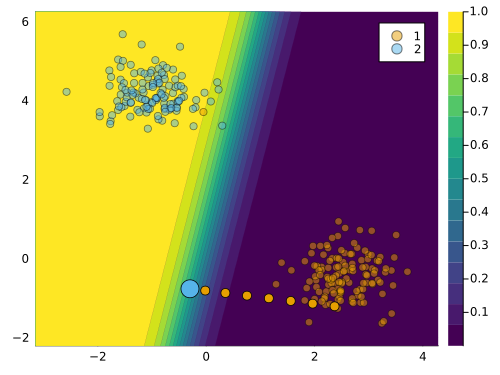
\includegraphics[width=3.33333in,height=2.5in]{www/ce_binary.png}

}

\caption{\label{fig-binary}Counterfactual path using generic
counterfactual generator for conventional binary classifier.}

\end{figure}%

In this simple example, the generic generator produces a valid
counterfactual, since the decision boundary is crossed and the predicted
label is flipped. But the counterfactual is not plausible: it does not
appear to be generated by the same DGP as the observed data in the
target class. This is because the generic generator does not take into
account any of the desiderata mentioned in Section~\ref{sec-method},
except for the distance to the factual sample.

\subsection{Composing Generators}\label{sec-gen-comp}

To address these issues, we can leverage the ideas underlying some of
the more advanced counterfactual generators introduced above. In
particular, we will now show how easy it is to
\href{https://juliatrustworthyai.github.io/CounterfactualExplanations.jl/v0.1/tutorials/generators/}{compose
custom generators} that blend different ideas through user-friendly
macros.

Suppose we wanted to address the desiderata of plausibility and
diversity. We could do this by blending ideas underlying the \emph{DiCE}
generator with the \emph{REVISE} generator. Formally, the corresponding
search objective would be defined as follows,

\begin{equation}\phantomsection\label{eq-comp}{
\mathbf{Z}^\prime = \arg \min_{\mathbf{Z}^\prime \in \mathcal{Z}^{L \times K}} \{  {\ell(M(f(\mathbf{Z}^\prime)),t)} + \lambda \cdot {\text{diversity}(f(\mathbf{Z}^\prime)) }  \} 
}\end{equation}

where \(\mathbf{X}^\prime\) is an \(L\)-dimensional array of
counterfactuals,
\(f: \mathcal{Z}^{L \times K} \mapsto \mathcal{X}^{L \times D}\) is a
function that maps the \(L \times K\)-dimensional latent space
\(\mathcal{Z}\) to the \(L \times D\)-dimensional feature space
\(\mathcal{X}\) and \(\text{diversity}(\cdot)\) is the penalty proposed
by Mothilal, Sharma, and Tan
(\citeproc{ref-mothilal2020explaining}{2020}) that induces diverse sets
of counterfactuals. As in Equation~\ref{eq-solution}, \(\ell\) is the
loss function, \(M\) is the black-box model, \(t\) is the target class,
and \(\lambda\) is the strength of the penalty.

Code \ref{lst:composed} demonstrates how Equation~\ref{eq-comp} can be
seamlessly translated into Julia code. We begin by instantiating a
\texttt{GradientBasedGenerator} in line \ref{line:composed-init}. Next,
we use chained macros for composition: firstly, we define the
counterfactual search \texttt{@objective} corresponding to \emph{DiCE}
in line \ref{line:composed-dice}; secondly, we define the latent space
search strategy corresponding to \emph{REVISE} using the
\texttt{@search\_latent\_space} macro in line
\ref{line:composed-latent}; finally, we specify our prefered
optimisation method using the \texttt{@with\_optimiser} macro in line
\ref{line:composed-adam}.

\begin{lstlisting}[language=Julia, escapechar=§, numbers=left, label={lst:composed}, caption={Composing a custom generator.}]
generator = GradientBasedGenerator() §\label{line:composed-init}§
@chain generator begin
    @objective logitcrossentropy 
      + 0.2ddp_diversity §\label{line:composed-dice}§
    @search_latent_space §\label{line:composed-latent}§
    @with_optimiser Adam(0.005) §\label{line:composed-adam}§
end
\end{lstlisting}

In this case, the counterfactual search is performed in the latent space
of a Variational Autoencoder (VAE) that is automatically trained on the
observed data. It is important to specify the keyword argument
\texttt{num\_counterfactuals} of the \texttt{generate\_counterfactual}
to some value higher than \(1\) (default), to ensure that the diversity
penalty is effective. The resulting counterfactual path is shown in
Figure~\ref{fig-binary-advanced} below. We observe that the resulting
counterfactuals are diverse and the majority of them are plausible.

\begin{figure}

\centering{

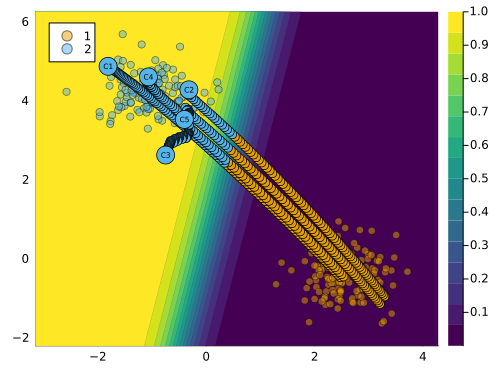
\includegraphics[width=3.33333in,height=2.5in]{www/binary_advanced.png}

}

\caption{\label{fig-binary-advanced}Counterfactual path using the
\emph{DiCE} generator.}

\end{figure}%

\subsection{Mutability Constraints}\label{sec-mut}

In practice, features usually cannot be perturbed arbitrarily. Suppose,
for example, that one of the features used by a bank to predict the
creditworthiness of its clients is \emph{age}. If a counterfactual
explanation for the prediction model indicates that older clients should
``grow younger'' to improve their creditworthiness, then this is an
interesting insight (it reveals age bias), but the provided recourse is
not actionable. In such cases, we may want to constrain the mutability
of features. To illustrate how this can be implemented in our package,
we will continue with the example from above.

Mutability can be defined in terms of four different options: 1) the
feature is mutable in both directions, 2) the feature can only increase
(e.g.~\emph{age}), 3) the feature can only decrease (e.g.~\emph{time
left} until your next deadline) and 4) the feature is not mutable
(e.g.~\emph{skin colour}, \emph{ethnicity}, \ldots). To specify which
category a feature belongs to, users can pass a vector of symbols
containing the mutability constraints at the pre-processing stage. For
each feature one can choose from these four options: \texttt{:both}
(mutable in both directions), \texttt{:increase} (only up),
\texttt{:decrease} (only down) and \texttt{:none} (immutable). By
default, \texttt{nothing} is passed to that keyword argument and it is
assumed that all features are mutable in both directions.\footnote{Mutability
  constraints are not yet implemented for Latent Space search.}

We can impose that the first feature is immutable as follows:
\texttt{counterfactual\_data.mutability\ =\ {[}:none,\ :both{]}}. The
resulting counterfactual path is shown in Figure~\ref{fig-mutability}
below. Since only the second feature can be perturbed, the sample can
only move along the vertical axis. In this case, the counterfactual
search does not yield a valid counterfactual, since the target class is
not reached.

\begin{figure}

\centering{

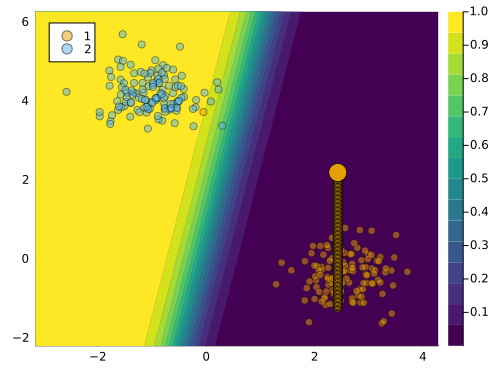
\includegraphics[width=3.33333in,height=2.5in]{www/constraint_mutability.png}

}

\caption{\label{fig-mutability}Counterfactual path with immutable
feature.}

\end{figure}%

\subsection{Evaluation and Benchmarking}\label{sec-eval}

The package also makes it easy to
\href{https://juliatrustworthyai.github.io/CounterfactualExplanations.jl/v0.1/tutorials/evaluation/}{evaluate}
counterfactuals with respect to many of the desiderata mentioned above.
For example, users may want to infer how costly the provided recourse is
to individuals. To this end, we can measure the distance of the
counterfactual from its original value. The API call to compute the
distance metric defined in Wachter, Mittelstadt, and Russell
(\citeproc{ref-wachter2017counterfactual}{2017}), for instance, is as
simple as \texttt{evaluate(ce;\ measure=distance\_mad)}, where
\texttt{ce} can also be a vector of \texttt{CounterfactualExplanation}s.

Additionally, the package provides a
\href{https://juliatrustworthyai.github.io/CounterfactualExplanations.jl/v0.1/tutorials/benchmarking/}{benchmarking}
framework that allows users to compare the performance of different
generators on a given dataset. In Figure~\ref{fig-bmk} we show the
results of a benchmark comparing several generators in terms of the
average cost and implausibility of the generated counterfactuals. The
cost is proxied by the L1-norm of the difference between the factual and
counterfactual features, while implausibility is measured by the
distance of the counterfactuals from samples in the target class. The
results illustrate that there is a tradeoff between minimizing costs to
individuals and generating plausible counterfactuals.

\begin{figure}

\centering{

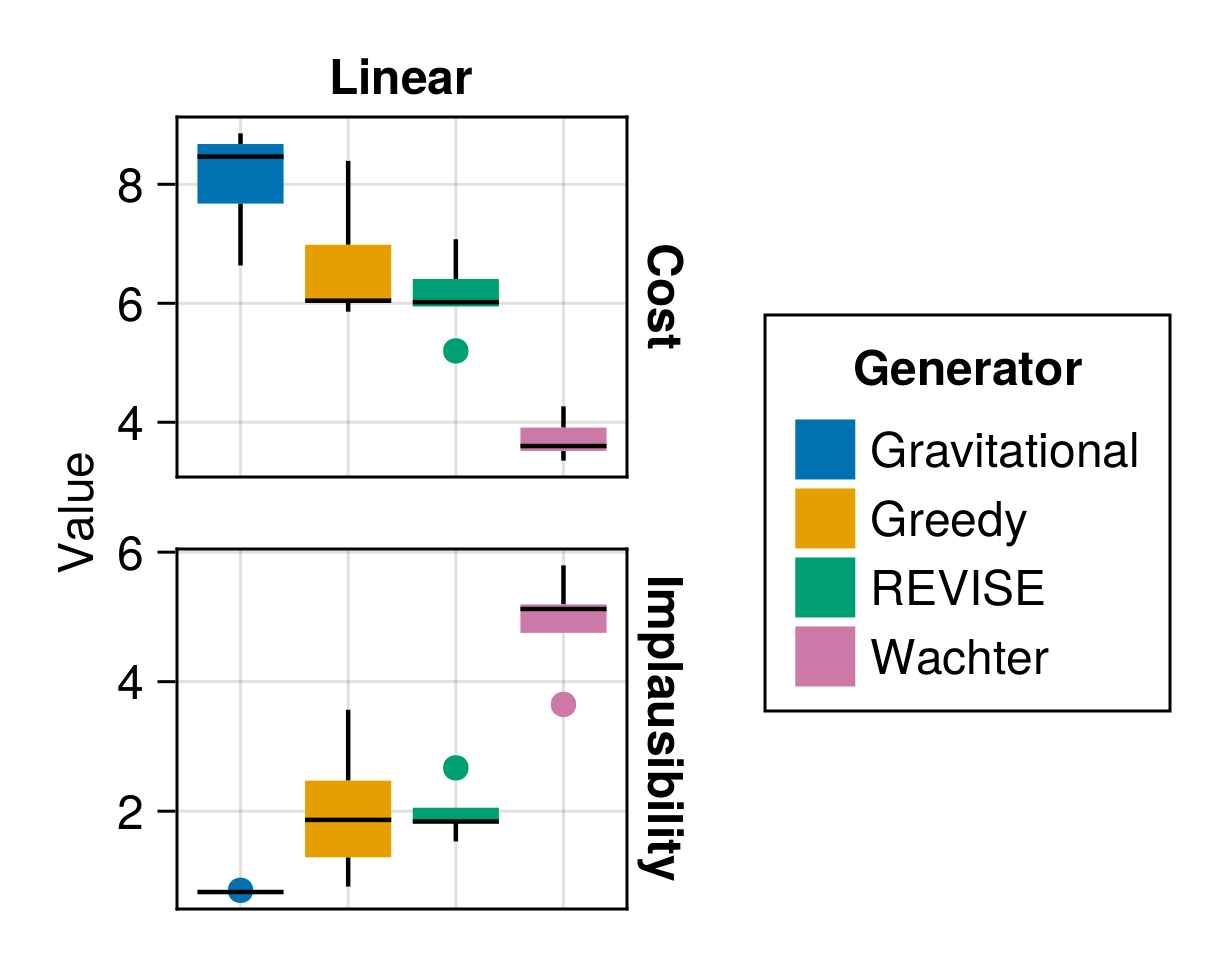
\includegraphics[width=3.33333in,height=2.5in]{www/bmk.png}

}

\caption{\label{fig-bmk}Benchmarking results for different generators.}

\end{figure}%

\section{Customization and Extensibility}\label{sec-custom}

One of our priorities has been to make our package customizable and
extensible. In the long term, we aim to add support for more default
models and counterfactual generators. In the short term, it is designed
to allow users to integrate models and generators themselves. These
community efforts will facilitate our long-term goals.

\subsection{Adding Custom Models}\label{sec-custom-mod}

At the high level, only two steps are necessary to make any supervised
learning model compatible with our package:

\begin{itemize}
\tightlist
\item
  \textbf{Subtyping}: We need to subtype the
  \texttt{AbstractFittedModel}.
\item
  \textbf{Dispatch}: The functions \texttt{logits} and \texttt{probs}
  need to be extended through custom methods for the model in question.
\end{itemize}

To demonstrate how this can be done in practice, we will reiterate here
how native support for \href{https://fluxml.ai/}{\texttt{Flux.jl}}
(\citeproc{ref-innes2018flux}{Innes 2018}) deep learning models was
enabled.\footnote{Flux models are now natively supported by our package
  and can be instantiated by calling \texttt{FluxModel()}.} Once again
we use synthetic data for an illustrative example. Code \ref{lst:nn}
below builds a simple model architecture that can be used for a
multi-class prediction task. Note how outputs from the final layer are
not passed through a softmax activation function, since the
counterfactual loss is evaluated with respect to logits as we discussed
earlier. The model is trained with dropout.

\begin{lstlisting}[language=Julia, escapechar=@, numbers=left, label={lst:nn}, caption={A simple neural network model.}]
n_hidden = 32
output_dim = length(unique(y))
input_dim = 2
model = Chain(
    Dense(input_dim, n_hidden, activation),
    Dropout(0.1),
    Dense(n_hidden, output_dim)
)  
\end{lstlisting}

Code \ref{lst:mymodel} below implements the two steps that were
necessary to make Flux models compatible with the package. In line
\ref{line:mymodel-subtype} we declare our new struct as a subtype of
\texttt{AbstractDifferentiableModel}, which itself is an abstract
subtype of \texttt{AbstractFittedModel}.\footnote{Note that in line
  \ref{line:mymodel-likelihood} we also provide a field determining the
  likelihood. This is optional and only used internally to determine
  which loss function to use in the counterfactual search. If this field
  is not provided to the model, the loss function needs to be explicitly
  supplied to the generator.} Computing logits amounts to just calling
the model on inputs. Predicted probabilities for labels can be computed
by passing logits through the softmax function.

\begin{lstlisting}[language=Julia, escapechar=@, numbers=left, label={lst:mymodel}, caption={A wrapper for Flux models.}]
# Step 1)
struct MyFluxModel <: AbstractDifferentiableModel @\label{line:mymodel-subtype}@
    model::Any
    likelihood::Symbol @\label{line:mymodel-likelihood}@
end

# Step 2)
# import functions in order to extend
import CounterfactualExplanations.Models: logits
import CounterfactualExplanations.Models: probs 
logits(M::MyFluxModel, X::AbstractArray) = M.model(X)
probs(M::MyFluxModel, X::AbstractArray) = softmax(logits(M, X))
M = MyFluxModel(model)
\end{lstlisting}

The API call for generating counterfactuals for our new model is the
same as before. Figure~\ref{fig-multi} shows the resulting
counterfactual path for a randomly chosen sample. In this case, the
contour shows the predicted probability that the input is in the target
class (\(t=2\)).

\begin{figure}

\centering{

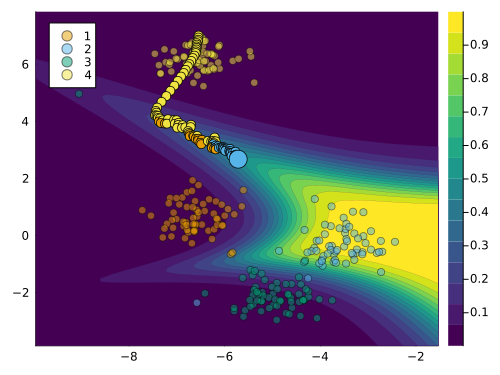
\includegraphics[width=3.33333in,height=2.5in]{www/ce_multi.png}

}

\caption{\label{fig-multi}Counterfactual path using generic
counterfactual generator for multi-class classifier.}

\end{figure}%

\subsection{Adding Custom Generators}\label{sec-custom-gen}

In some cases, composability may not be sufficient to implement specific
logics underlying certain counterfactual generators. In such cases,
users may want to implement custom generators. To illustrate how this
can be done we will consider a simple extension of our
\texttt{GenericGenerator}. As we have seen above, Counterfactual
Explanations are not unique. In light of this, we might be interested in
quantifying the uncertainty around the generated counterfactuals
(\citeproc{ref-delaney2021uncertainty}{Delaney, Greene, and Keane
2021}). One idea could be, to use dropout to randomly switch features on
and off in each iteration. Without dwelling further on the merit of this
idea, we will now briefly show how this can be implemented.

\subsubsection{A Generator with Dropout}\label{a-generator-with-dropout}

Code \ref{lst:dropout} below implements two important steps: 1) create
an abstract subtype of the \texttt{AbstractGradientBasedGenerator} and
2) create a constructor with an additional field for the dropout
probability.

\begin{lstlisting}[language=Julia, escapechar=@, numbers=left, label={lst:dropout}, caption={Building a custom generator with dropout.}]
# Abstract suptype:
abstract type AbstractDropoutGenerator <: AbstractGradientBasedGenerator end
# Constructor:
struct DropoutGenerator <: AbstractDropoutGenerator
    loss::Symbol # loss function
    complexity::Function # complexity function
    @$\lambda$@::AbstractFloat # strength of penalty
    decision_threshold::Union{Nothing,AbstractFloat} 
    opt::Any # optimizer
    @$\tau$@::AbstractFloat # tolerance for convergence
    p_dropout::AbstractFloat # dropout rate
end
\end{lstlisting}

Next, in Code \ref{lst:generate} we define how feature perturbations are
generated for our custom dropout generator: in particular, we extend the
relevant function through a method that implements the dropout logic.

\begin{lstlisting}[language=Julia, escapechar=@, numbers=left, label={lst:generate}, caption={Generating feature perturbations with dropout.}]
using CounterfactualExplanations.Generators
function Generators.generate_perturbations(
    generator::AbstractDropoutGenerator, 
    ce::CouterfactualExplanation
)
    @$s^\prime$@ = deepcopy(ce.@$s^\prime$@)
    new_@$s^\prime$@ = Generators.propose_state(
        generator, ce)
    @$\Delta s^\prime$@ = new_@$s^\prime$@ - @$s^\prime$@ # gradient step
    # Dropout:
    set_to_zero = sample(
        1:length(@$\Delta s^\prime$@),
        Int(round(generator.p_dropout*length(@$\Delta s^\prime$@))),
        replace=false
    )
    @$\Delta s^\prime$@[set_to_zero] .= 0
    return @$\Delta s^\prime$@
end
\end{lstlisting}

Finally, we proceed to generate counterfactuals in the same way we
always do. The resulting counterfactual path is shown in
Figure~\ref{fig-dropout}.

\begin{figure}

\centering{

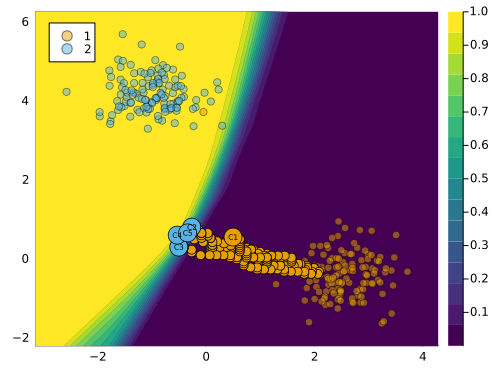
\includegraphics[width=3.33333in,height=2.5in]{www/dropout.png}

}

\caption{\label{fig-dropout}Counterfactual path for a generator with
dropout.}

\end{figure}%

\section{A Real-World Examples}\label{sec-emp}

Now that we have explained the basic functionality of
\texttt{CounterfactualExplanations.jl} through some synthetic examples,
it is time to work through examples involving real-world data.

\subsection{Give Me Some Credit}\label{give-me-some-credit}

The \emph{Give Me Some Credit} dataset is one of the tabular real-world
datasets that ship with the package
(\citeproc{ref-kaggle2011give}{Kaggle 2011}). It can be used to train a
binary classifier to predict whether a borrower is likely to experience
financial difficulties in the next two years. In particular, we have an
output variable \(y \in \{0=\texttt{no stress},1=\texttt{stress}\}\) and
a feature matrix \(X\) that includes socio-demographic variables like
\texttt{age} and \texttt{income}. A retail bank might use such a
classifier to determine if potential borrowers should receive credit or
not.

For the classification task, we use a Multi-Layer Perceptron with
dropout regularization. Using the Gravitational generator
(\citeproc{ref-altmeyer2023endogenous}{Altmeyer et al. 2023}) we will
generate counterfactuals for ten randomly chosen individuals that would
be denied credit based on our pre-trained model. Concerning the
mutability of features, we only impose that the \texttt{age} cannot be
decreased.

Figure~\ref{fig-credit} shows the resulting counterfactuals proposed by
Wachter in the two-dimensional feature space spanned by the \texttt{age}
and \texttt{income} variables. An increase in income and age is
recommended for the majority of individuals, which seems plausible: both
age and income are typically positively related to creditworthiness.

\begin{figure}

\centering{

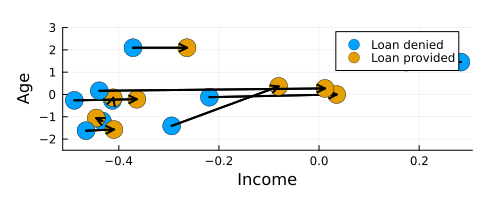
\includegraphics[width=3.33333in,height=1.33333in]{www/credit.png}

}

\caption{\label{fig-credit}Give Me Some Credit: counterfactuals for
would-be borrowers proposed by the Gravitational Generator.}

\end{figure}%

\subsection{MNIST}\label{mnist}

For our second example, we will look at image data. The MNIST dataset
contains 60,000 training samples of handwritten digits in the form of
28x28 pixel grey-scale images (\citeproc{ref-lecun1998mnist}{LeCun
1998}). Each image is associated with a label indicating the digit (0-9)
that the image represents. The data makes for an interesting case study
of CE because humans have a good idea of what plausible counterfactuals
of digits look like. For example, if you were asked to pick up an eraser
and turn the digit in the left panel of Figure~\ref{fig-mnist} into a
four (4) you would know exactly what to do: just erase the top part.

On the model side, we will use a simple multi-layer perceptron (MLP).
Code \ref{lst:mnist-setup} loads the data and the pre-trained MLP. It
also loads two pre-trained Variational Auto-Encoders, which will be used
by our counterfactual generator of choice for this task: \emph{REVISE}.

\begin{lstlisting}[language=Julia, escapechar=@, numbers=left, label={lst:mnist-setup}, caption={Loading pre-trained models and data for MNIST.}]
counterfactual_data = load_mnist()
X, y = unpack_data(counterfactual_data)
input_dim, n_obs = size(counterfactual_data.X)
M = load_mnist_mlp()
vae = load_mnist_vae()
vae_weak = load_mnist_vae(;strong=false)
\end{lstlisting}

The proposed counterfactuals are shown in Figure~\ref{fig-mnist}. In the
case in which \emph{REVISE} has access to an expressive VAE (centre),
the result looks convincing: the perturbed image does look like it
represents a four (4). In terms of explainability, we may conclude that
removing the top part of the handwritten nine (9) leads the black-box
model to predict that the perturbed image represents a four (4). We
should note, however, that the quality of counterfactuals produced by
\emph{REVISE} hinges on the performance of the underlying generative
model, as demonstrated by the result on the right. In this case,
\emph{REVISE} uses a weak VAE and the resulting counterfactual is
invalid. In light of this, we recommend using Latent Space search with
care.

\begin{figure}

\centering{

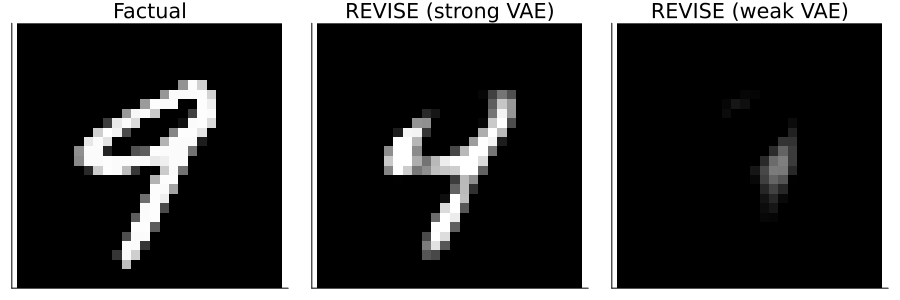
\includegraphics[width=3.33333in,height=1.11111in]{www/mnist_9to4_latent.png}

}

\caption{\label{fig-mnist}Counterfactual explanations for MNIST using a
Latent Space generator: turning a nine (9) into a four (4).}

\end{figure}%

\section{Discussion and Outlook}\label{sec-outlook}

We believe that this package in its current form offers a valuable
contribution to ongoing efforts towards XAI in Julia. That being said,
there is significant scope for future developments, which we briefly
outline in this final section.

\subsection{Candidate models and
generators}\label{candidate-models-and-generators}

The package supports various models and generators either natively or
through minimal augmentation. In future work, we would like to
prioritize the addition of further predictive models and generators.
Concerning the former, it would be useful to add native support for any
supervised models built in \texttt{MLJ.jl}, an extensive Machine
Learning framework for Julia (\citeproc{ref-blaom2020mlj}{Blaom et al.
2020}). This may also involve adding support for regression models as
well as additional non-differentiable models. In terms of counterfactual
generators, there is a list of recent methodologies that we would like
to implement including MINT
(\citeproc{ref-karimi2021algorithmic}{Karimi, Schölkopf, and Valera
2021}), ROAR (\citeproc{ref-upadhyay2021robust}{Upadhyay, Joshi, and
Lakkaraju 2021}) and FACE (\citeproc{ref-poyiadzi2020face}{Poyiadzi et
al. 2020}).

\subsection{Additional datasets}\label{additional-datasets}

For benchmarking and testing purposes it will be crucial to add more
datasets to our library. We have so far prioritized tabular datasets
that have typically been used in the literature on counterfactual
explanations including \emph{Adult}, \emph{Give Me Some Credit} and
\emph{German Credit} (\citeproc{ref-karimi2020survey}{Karimi, Barthe, et
al. 2020}). There is scope for adding data sources that have so far not
been explored much in this context including additional image datasets
as well as audio, natural language and time-series data.

\section{Concluding remarks}\label{sec-conclude}

\texttt{CounterfactualExplanation.jl} is a package for generating
Counterfactual Explanations and Algorithmic Recourse in Julia. Through
various synthetic and real-world examples, we have demonstrated the
basic usage of the package as well as its extensibility. The package has
already served us in our research to benchmark various methodological
approaches to Counterfactual Explanations and Algorithmic Recourse. We
therefore strongly believe that it should help other practitioners and
researchers in their own efforts towards Trustworthy AI.

We envision this package to one day constitute the go-to place for
explaining arbitrary predictive models through an extensive suite of
counterfactual generators. As a major next step, we aim to make our
library as compatible as possible with the popular
\href{https://alan-turing-institute.github.io/MLJ.jl/dev/}{\texttt{MLJ.jl}}
package for machine learning in Julia. We invite the Julia community to
contribute to these goals through usage, open challenge and active
development.

\section{Acknowledgements}\label{sec-ack}

We are immensely grateful to the group of TU Delft students who
contributed huge improvements to this package as part of a university
project in 2023: Rauno Arike, Simon Kasdorp, Lauri Kesküll, Mariusz
Kicior, Vincent Pikand. We also want to thank the broader Julia
community for being welcoming and open and for supporting research
contributions like this one. Some of the members of TU Delft were
partially funded by ICAI AI for Fintech Research, an ING---TU Delft
collaboration.

\section*{References}\label{references}
\addcontentsline{toc}{section}{References}

\phantomsection\label{refs}
\begin{CSLReferences}{1}{0}
\bibitem[\citeproctext]{ref-altmeyer2023endogenous}
Altmeyer, Patrick, Giovan Angela, Aleksander Buszydlik, Karol Dobiczek,
Arie van Deursen, and Cynthia Liem. 2023. {``Endogenous {Macrodynamics}
in {Algorithmic} {Recourse}.''} In \emph{First {IEEE} {Conference} on
{Secure} and {Trustworthy} {Machine} {Learning}}.
\url{https://doi.org/10.1109/satml54575.2023.00036}.

\bibitem[\citeproctext]{ref-antoran2020getting}
Antorán, Javier, Umang Bhatt, Tameem Adel, Adrian Weller, and José
Miguel Hernández-Lobato. 2020. {``Getting a Clue: {A} Method for
Explaining Uncertainty Estimates.''}
\url{https://arxiv.org/abs/2006.06848}.

\bibitem[\citeproctext]{ref-arrieta2020explainable}
Arrieta, Alejandro Barredo, Natalia Diaz-Rodriguez, Javier Del Ser,
Adrien Bennetot, Siham Tabik, Alberto Barbado, Salvador Garcia, et al.
2020. {``Explainable {Artificial Intelligence} ({XAI}): {Concepts},
Taxonomies, Opportunities and Challenges Toward Responsible {AI}.''}
\emph{Information Fusion} 58: 82--115.
\url{https://doi.org/10.1016/j.inffus.2019.12.012}.

\bibitem[\citeproctext]{ref-becker1996adult}
Barry Becker, Ronny Kohavi. 1996. {``Adult.''} UCI Machine Learning
Repository. \url{https://doi.org/10.24432/C5XW20}.

\bibitem[\citeproctext]{ref-blaom2020mlj}
Blaom, Anthony D., Franz Kiraly, Thibaut Lienart, Yiannis Simillides,
Diego Arenas, and Sebastian J. Vollmer. 2020. {``{MLJ}: {A Julia}
Package for Composable Machine Learning.''} \emph{Journal of Open Source
Software} 5 (55): 2704. \url{https://doi.org/10.21105/joss.02704}.

\bibitem[\citeproctext]{ref-borch2022machine}
Borch, Christian. 2022. {``Machine Learning, Knowledge Risk, and
Principal-Agent Problems in Automated Trading.''} \emph{Technology in
Society}, 101852. \url{https://doi.org/10.1016/j.techsoc.2021.101852}.

\bibitem[\citeproctext]{ref-buolamwini2018gender}
Buolamwini, Joy, and Timnit Gebru. 2018. {``Gender Shades:
{Intersectional} Accuracy Disparities in Commercial Gender
Classification.''} In \emph{Conference on Fairness, Accountability and
Transparency}, 77--91. {PMLR}.

\bibitem[\citeproctext]{ref-dandl2023counterfactuals}
Dandl, Susanne, Andreas Hofheinz, Martin Binder, Bernd Bischl, and
Giuseppe Casalicchio. 2023. {``Counterfactuals: {An} {R} {Package} for
{Counterfactual} {Explanation} {Methods}.''} arXiv.
\url{http://arxiv.org/abs/2304.06569}.

\bibitem[\citeproctext]{ref-delaney2021uncertainty}
Delaney, Eoin, Derek Greene, and Mark T. Keane. 2021. {``Uncertainty
{Estimation} and {Out}-of-{Distribution} {Detection} for
{Counterfactual} {Explanations}: {Pitfalls} and {Solutions}.''} arXiv.
\url{http://arxiv.org/abs/2107.09734}.

\bibitem[\citeproctext]{ref-fan2020interpretability}
Fan, Fenglei, Jinjun Xiong, and Ge Wang. 2020. {``On Interpretability of
Artificial Neural Networks.''} \url{https://arxiv.org/abs/2001.02522}.

\bibitem[\citeproctext]{ref-goodfellow2014explaining}
Goodfellow, Ian J, Jonathon Shlens, and Christian Szegedy. 2014.
{``Explaining and Harnessing Adversarial Examples.''}
\url{https://arxiv.org/abs/1412.6572}.

\bibitem[\citeproctext]{ref-hoffman1994german}
Hoffman, Hans. 1994. {``German {Credit Data}.''}
\url{https://archive.ics.uci.edu/ml/datasets/statlog+(german+credit+data)}.

\bibitem[\citeproctext]{ref-innes2018flux}
Innes, Mike. 2018. {``Flux: {Elegant} Machine Learning with {Julia}.''}
\emph{Journal of Open Source Software} 3 (25): 602.
\url{https://doi.org/10.21105/joss.00602}.

\bibitem[\citeproctext]{ref-joshi2019realistic}
Joshi, Shalmali, Oluwasanmi Koyejo, Warut Vijitbenjaronk, Been Kim, and
Joydeep Ghosh. 2019. {``Towards Realistic Individual Recourse and
Actionable Explanations in Black-Box Decision Making Systems.''}
\url{https://arxiv.org/abs/1907.09615}.

\bibitem[\citeproctext]{ref-kaggle2011give}
Kaggle. 2011. {``Give Me Some Credit, {Improve} on the State of the Art
in Credit Scoring by Predicting the Probability That Somebody Will
Experience Financial Distress in the Next Two Years.''} {Kaggle}.
\url{https://www.kaggle.com/c/GiveMeSomeCredit}.

\bibitem[\citeproctext]{ref-karimi2020survey}
Karimi, Amir-Hossein, Gilles Barthe, Bernhard Schölkopf, and Isabel
Valera. 2020. {``A Survey of Algorithmic Recourse: Definitions,
Formulations, Solutions, and Prospects.''}
\url{https://arxiv.org/abs/2010.04050}.

\bibitem[\citeproctext]{ref-karimi2021algorithmic}
Karimi, Amir-Hossein, Bernhard Schölkopf, and Isabel Valera. 2021.
{``Algorithmic Recourse: From Counterfactual Explanations to
Interventions.''} In \emph{Proceedings of the 2021 {ACM Conference} on
{Fairness}, {Accountability}, and {Transparency}}, 353--62.

\bibitem[\citeproctext]{ref-karimi2020algorithmic}
Karimi, Amir-Hossein, Julius Von Kügelgen, Bernhard Schölkopf, and
Isabel Valera. 2020. {``Algorithmic Recourse Under Imperfect Causal
Knowledge: A Probabilistic Approach.''}
\url{https://arxiv.org/abs/2006.06831}.

\bibitem[\citeproctext]{ref-kaur2020interpreting}
Kaur, Harmanpreet, Harsha Nori, Samuel Jenkins, Rich Caruana, Hanna
Wallach, and Jennifer Wortman Vaughan. 2020. {``Interpreting
Interpretability: Understanding Data Scientists' Use of Interpretability
Tools for Machine Learning.''} In \emph{Proceedings of the 2020 {CHI}
Conference on Human Factors in Computing Systems}, 1--14.
\url{https://doi.org/10.1145/3313831.3376219}.

\bibitem[\citeproctext]{ref-krizhevsky2009learning}
Krizhevsky, A. 2009. {``Learning {Multiple} {Layers} of {Features} from
{Tiny} {Images}.''} In.
\url{https://www.semanticscholar.org/paper/Learning-Multiple-Layers-of-Features-from-Tiny-Krizhevsky/5d90f06bb70a0a3dced62413346235c02b1aa086}.

\bibitem[\citeproctext]{ref-lakshminarayanan2016simple}
Lakshminarayanan, Balaji, Alexander Pritzel, and Charles Blundell. 2016.
{``Simple and Scalable Predictive Uncertainty Estimation Using Deep
Ensembles.''} \url{https://arxiv.org/abs/1612.01474}.

\bibitem[\citeproctext]{ref-laugel2017inversea}
Laugel, Thibault, Marie-Jeanne Lesot, Christophe Marsala, Xavier Renard,
and Marcin Detyniecki. 2017. {``Inverse {Classification} for
{Comparison}-Based {Interpretability} in {Machine} {Learning}.''} arXiv.
\url{https://doi.org/10.48550/arXiv.1712.08443}.

\bibitem[\citeproctext]{ref-lecun1998mnist}
LeCun, Yann. 1998. {``The {MNIST} Database of Handwritten Digits.''}

\bibitem[\citeproctext]{ref-miller2019explanation}
Miller, Tim. 2019. {``Explanation in Artificial Intelligence: {Insights}
from the Social Sciences.''} \emph{Artificial Intelligence} 267: 1--38.
\url{https://doi.org/10.1016/j.artint.2018.07.007}.

\bibitem[\citeproctext]{ref-molnar2020interpretable}
Molnar, Christoph. 2020. \emph{Interpretable Machine Learning}. {Lulu.
com}.

\bibitem[\citeproctext]{ref-mothilal2020explaining}
Mothilal, Ramaravind K, Amit Sharma, and Chenhao Tan. 2020.
{``Explaining Machine Learning Classifiers Through Diverse
Counterfactual Explanations.''} In \emph{Proceedings of the 2020
{Conference} on {Fairness}, {Accountability}, and {Transparency}},
607--17. \url{https://doi.org/10.1145/3351095.3372850}.

\bibitem[\citeproctext]{ref-oneil2016weapons}
O'Neil, Cathy. 2016. \emph{Weapons of Math Destruction: {How} Big Data
Increases Inequality and Threatens Democracy}. {Crown}.

\bibitem[\citeproctext]{ref-pace1997sparse}
Pace, R Kelley, and Ronald Barry. 1997. {``Sparse Spatial
Autoregressions.''} \emph{Statistics \& Probability Letters} 33 (3):
291--97. \url{https://doi.org/10.1016/s0167-7152(96)00140-x}.

\bibitem[\citeproctext]{ref-pawelczyk2021carla}
Pawelczyk, Martin, Sascha Bielawski, Johannes van den Heuvel, Tobias
Richter, and Gjergji Kasneci. 2021. {``Carla: A Python Library to
Benchmark Algorithmic Recourse and Counterfactual Explanation
Algorithms.''} \url{https://arxiv.org/abs/2108.00783}.

\bibitem[\citeproctext]{ref-pawelczyk2022probabilistically}
Pawelczyk, Martin, Teresa Datta, Johannes van-den-Heuvel, Gjergji
Kasneci, and Himabindu Lakkaraju. 2022. {``Probabilistically {Robust}
{Recourse}: {Navigating} the {Trade}-Offs Between {Costs} and
{Robustness} in {Algorithmic} {Recourse}.''} \emph{arXiv Preprint
arXiv:2203.06768}.

\bibitem[\citeproctext]{ref-poyiadzi2020face}
Poyiadzi, Rafael, Kacper Sokol, Raul Santos-Rodriguez, Tijl De Bie, and
Peter Flach. 2020. {``{FACE}: {Feasible} and Actionable Counterfactual
Explanations.''} In \emph{Proceedings of the {AAAI}/{ACM Conference} on
{AI}, {Ethics}, and {Society}}, 344--50.

\bibitem[\citeproctext]{ref-rudin2019stop}
Rudin, Cynthia. 2019. {``Stop Explaining Black Box Machine Learning
Models for High Stakes Decisions and Use Interpretable Models
Instead.''} \emph{Nature Machine Intelligence} 1 (5): 206--15.
\url{https://doi.org/10.1038/s42256-019-0048-x}.

\bibitem[\citeproctext]{ref-schut2021generating}
Schut, Lisa, Oscar Key, Rory Mc Grath, Luca Costabello, Bogdan
Sacaleanu, Yarin Gal, et al. 2021. {``Generating {Interpretable
Counterfactual Explanations By Implicit Minimisation} of {Epistemic} and
{Aleatoric Uncertainties}.''} In \emph{International {Conference} on
{Artificial Intelligence} and {Statistics}}, 1756--64. {PMLR}.

\bibitem[\citeproctext]{ref-slack2021counterfactual}
Slack, Dylan, Anna Hilgard, Himabindu Lakkaraju, and Sameer Singh. 2021.
{``Counterfactual Explanations Can Be Manipulated.''} \emph{Advances in
Neural Information Processing Systems} 34.

\bibitem[\citeproctext]{ref-slack2020fooling}
Slack, Dylan, Sophie Hilgard, Emily Jia, Sameer Singh, and Himabindu
Lakkaraju. 2020. {``Fooling Lime and Shap: {Adversarial} Attacks on Post
Hoc Explanation Methods.''} In \emph{Proceedings of the {AAAI}/{ACM
Conference} on {AI}, {Ethics}, and {Society}}, 180--86.

\bibitem[\citeproctext]{ref-tolomei2017interpretable}
Tolomei, Gabriele, Fabrizio Silvestri, Andrew Haines, and Mounia Lalmas.
2017. {``Interpretable {Predictions} of {Tree}-Based {Ensembles} via
{Actionable} {Feature} {Tweaking}.''} In \emph{Proceedings of the 23rd
{ACM} {SIGKDD} {International} {Conference} on {Knowledge} {Discovery}
and {Data} {Mining}}, 465--74.
\url{https://doi.org/10.1145/3097983.3098039}.

\bibitem[\citeproctext]{ref-upadhyay2021robust}
Upadhyay, Sohini, Shalmali Joshi, and Himabindu Lakkaraju. 2021.
{``Towards {Robust} and {Reliable Algorithmic Recourse}.''}
\url{https://arxiv.org/abs/2102.13620}.

\bibitem[\citeproctext]{ref-ustun2019actionable}
Ustun, Berk, Alexander Spangher, and Yang Liu. 2019. {``Actionable
Recourse in Linear Classification.''} In \emph{Proceedings of the
{Conference} on {Fairness}, {Accountability}, and {Transparency}},
10--19. \url{https://doi.org/10.1145/3287560.3287566}.

\bibitem[\citeproctext]{ref-varshney2022trustworthy}
Varshney, Kush R. 2022. \emph{Trustworthy {Machine Learning}}.
{Chappaqua, NY, USA}: {Independently Published}.

\bibitem[\citeproctext]{ref-verma2020counterfactual}
Verma, Sahil, John Dickerson, and Keegan Hines. 2020. {``Counterfactual
Explanations for Machine Learning: {A} Review.''}
\url{https://arxiv.org/abs/2010.10596}.

\bibitem[\citeproctext]{ref-wachter2017counterfactual}
Wachter, Sandra, Brent Mittelstadt, and Chris Russell. 2017.
{``Counterfactual Explanations Without Opening the Black Box:
{Automated} Decisions and the {GDPR}.''} \emph{Harv. JL \& Tech.} 31:
841. \url{https://doi.org/10.2139/ssrn.3063289}.

\bibitem[\citeproctext]{ref-xiao2017fashion}
Xiao, Han, Kashif Rasul, and Roland Vollgraf. 2017. {``Fashion-{MNIST}:
A {Novel} {Image} {Dataset} for {Benchmarking} {Machine} {Learning}
{Algorithms}.''} arXiv. \url{https://doi.org/10.48550/arXiv.1708.07747}.

\bibitem[\citeproctext]{ref-yeh2009comparisons}
Yeh, I-Cheng, and Che-hui Lien. 2009. {``The Comparisons of Data Mining
Techniques for the Predictive Accuracy of Probability of Default of
Credit Card Clients.''} \emph{Expert Systems with Applications} 36 (2):
2473--80. \url{https://doi.org/10.1016/j.eswa.2007.12.020}.

\end{CSLReferences}



\end{document}
